%%%%%%%%%%%%%%%%%%%%%%%%%%%%%%%%%%%%%%%%%%

\chapter{Ramsey method demonstration in prototype apparatus}\label{chap:lanl_ramsey_demonstration}

%%%%%%%%%%%%%%%%%%%%%%%%%%%%%%%%%%%%%%%%%%

This chapter summarizes a series of measurements taken on the North beamline in 2017 with an early prototype of the nEDM apparatus in a 2-layer \acrshort{msr} (Fig.~\ref{fig:ramsey_2017_apparatus}). Rabi and Ramsey fringes were produced, and measurements of spin relaxation lifetimes $T_1$ and $T_2$ were performed. 

%%%%%%%%%%%%%%%%%%%%%%%%%%%%%%%%%%%%%%%%%%%%%%

\section{Description of experimental setup (2017)}

%%%%%%%%%%%%%%%%%%%%%%%%%%%%%%%%%%%%%%%%%%%%%%


\begin{figure}[hb]
\centering
\begin{minipage}{.45\textwidth}
    \centering
    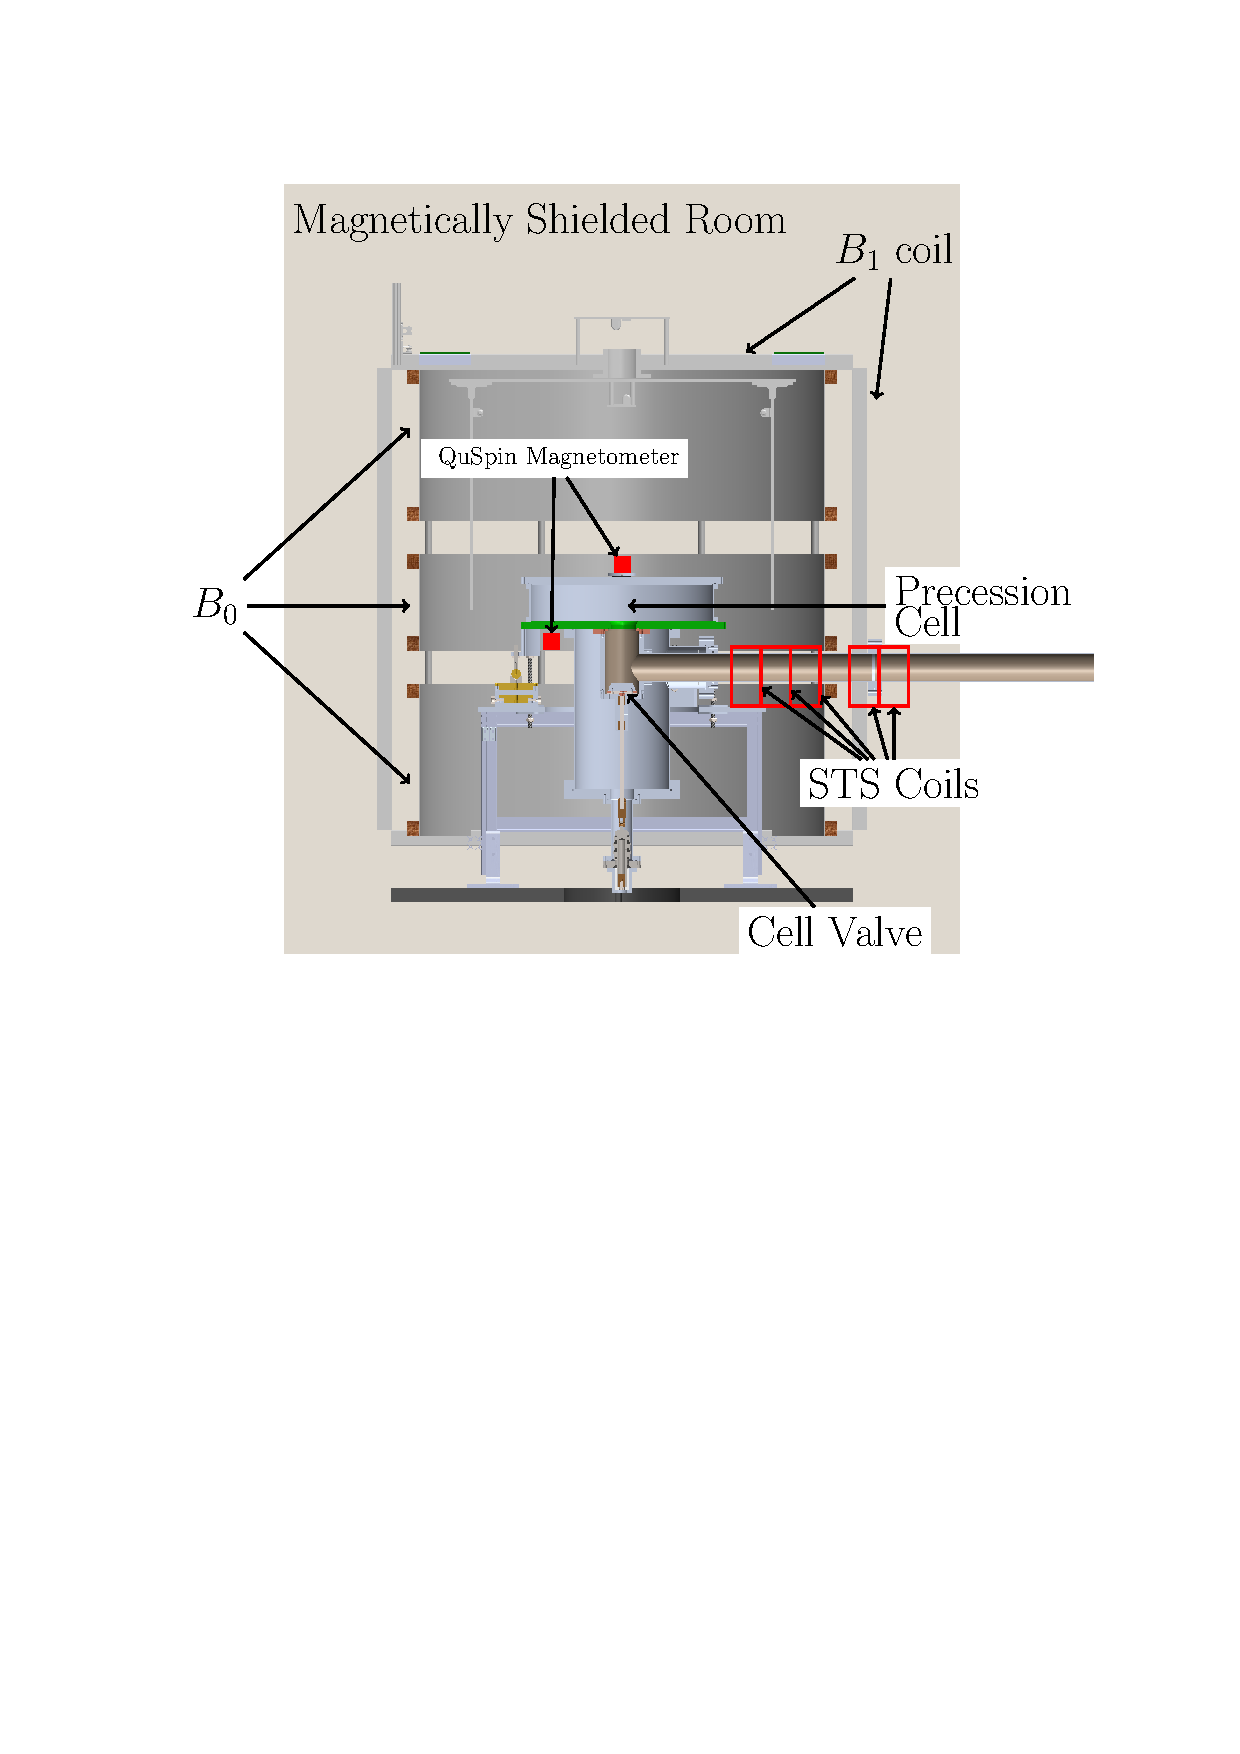
\includegraphics[width=\textwidth]{figures/ramsey2017_apparatus.pdf}
    \caption
    [Prototype experimental apparatus for measurements performed in 2017.]
    {Prototype experimental apparatus for measurements performed in 2017. Figure courtesy of Takeyasu Ito.}
    \label{fig:ramsey_2017_apparatus}
\end{minipage}%
\hspace{10pt}
\begin{minipage}{.45\textwidth}
    \centering
    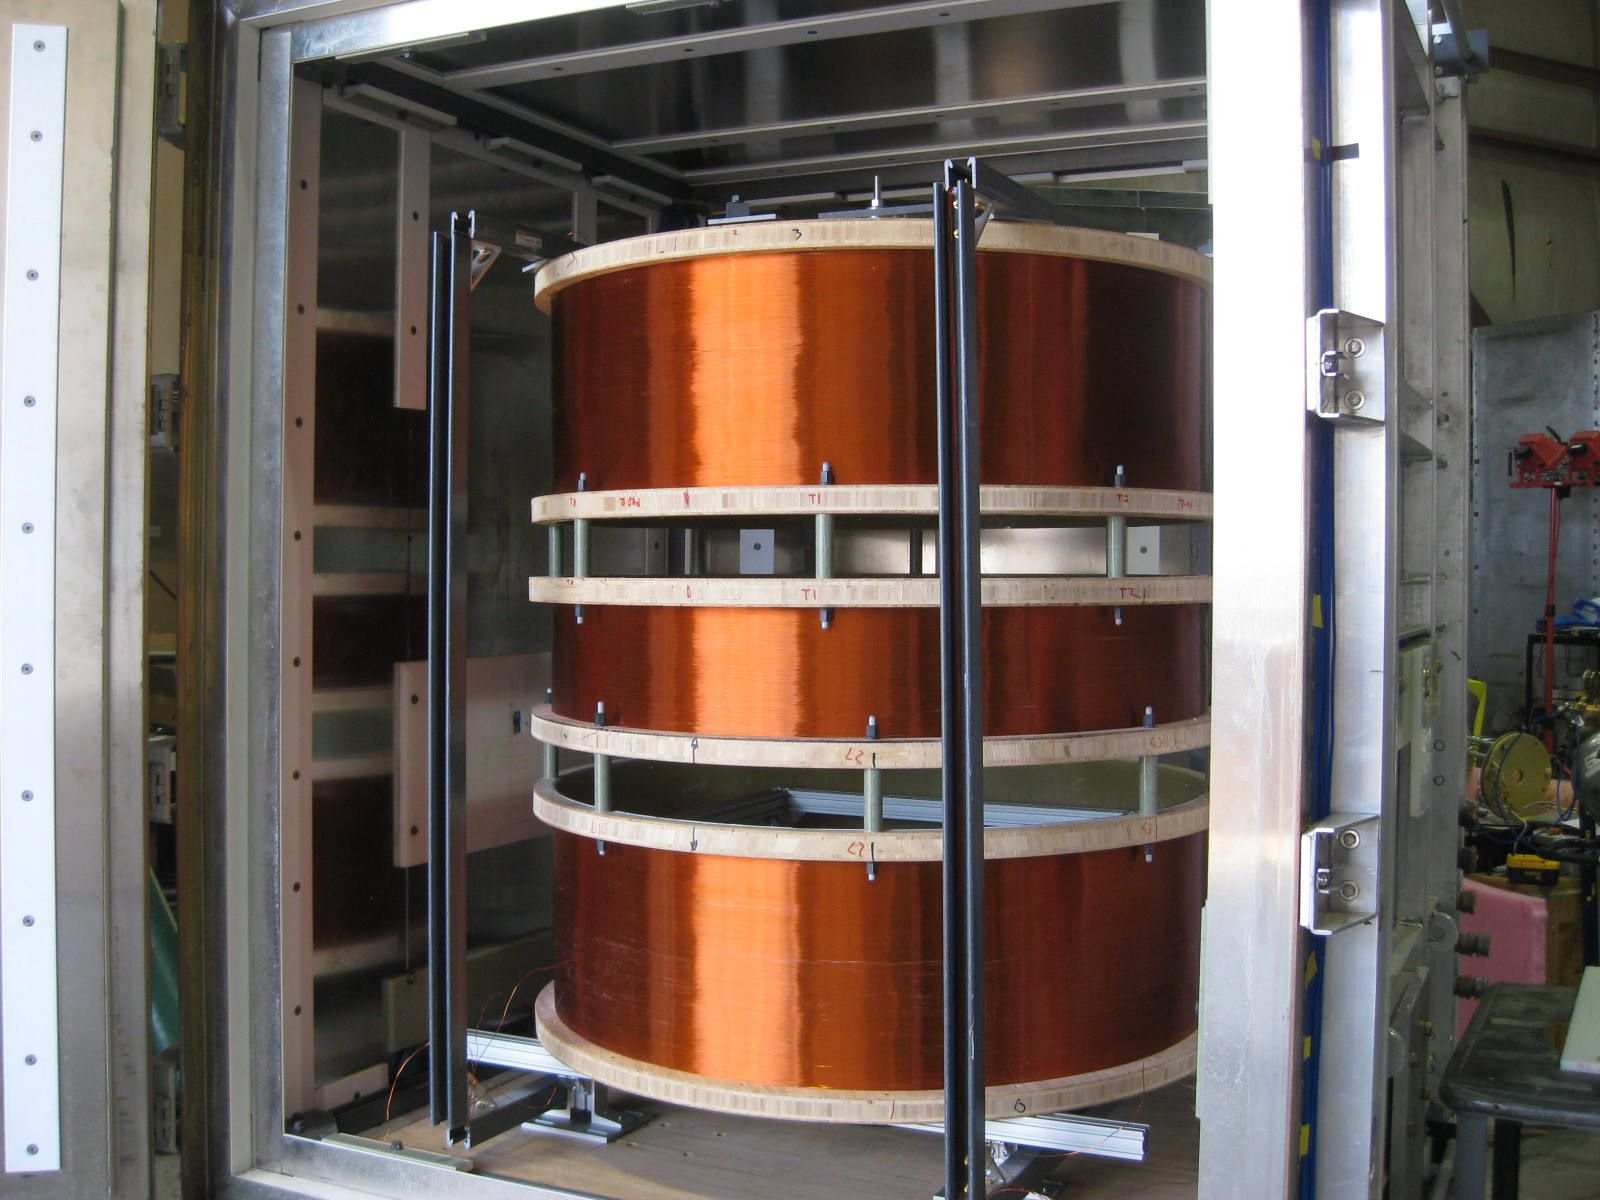
\includegraphics[width=0.9\textwidth]{figures/ramsey2017_B0_coil.jpg}
    \caption
    {$B_0$ coil prototype in the 2-layer MSR}
    \label{fig:ramsey_2017_B0_coil_prototype}
\end{minipage}
\end{figure}

Excepting the magnetic environment, the North beamline configuration in 2017 was largely equivalent to run condition 4 from Tab.~\ref{tb:runconditions} (layout depicted in Fig.~\ref{fig:NorthBeamlineLayout}), where the cell with dPS-walls, NiP electrode prototypes, rotary switcher, and drop detector used were the same as in Chap.~\ref{chap:north_beamline_paper}. For the 2017 measurement cycle, the window in the \acrshort{pm} region was comprised of \qty{50.8}{\micro\meter}-thick Al 5052 and the precession cell was housed in a 2-layer MSR. The 2-layer MSR reduced the ambient magnetic field to $\leq \qty{50}{nT}$. Two QuSpin Total Field magnetometers (sensitivity of $<\qty{1}{pT\per\sqrt{Hz}}$ in the 0.1--\qty{100}{\hertz} range) were used for field monitoring, one above the precession cell and one below. The magnetometers and MSR were later repurposed for the magnetic impurity scanner (Sec.~\ref{sec:magnetic_impurity_scanner}).

%%%%%%%%%%%%%%%%%%%%%%%%%%%%%%%%%%%%%%%%%%%%%%

\subsection
{
    \texorpdfstring{$B_0$ and transport coils}
                    {B0 and transport coils}
}

%%%%%%%%%%%%%%%%%%%%%%%%%%%%%%%%%%%%%%%%%%%%%%

\begin{figure}
    \centering
    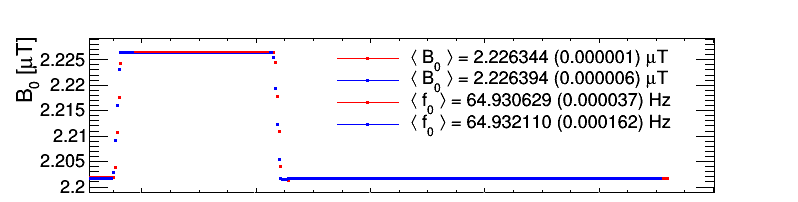
\includegraphics[width=0.8\textwidth]{figures/ramsey2017_B0.png}
    \caption
    [$|B_0|$ measured by the magnetometer located above the precession cell.]
    {$|B_0|$ measured by the magnetometer located above the precession cell. Blue and red lines refer to the measurement pair illustrated in Fig.~\ref{subfig:ramsey2017_t1_doublet}. The field drift between the two measurement periods was $\Delta B_0\approx\qty{50}{pT}$. When the STS transport coils were on during the fill and cell dump periods, $B_0\approx\qty{2.02}{\micro T}$.  During the measurement periods, $B_0\approx\qty{2.226}{\micro T}$. Figure courtesy of Robert Pattie Jr.}
    \label{fig:ramsey_2017_b0_map}
\end{figure}

An early prototype of the $B_0$ coil was constructed from 18 AWG copper wire wound about cylindrical fiberglass-reinforced plastic frames (Fig.~\ref{fig:ramsey_2017_B0_coil_prototype}). The design was based on the gapped solenoid in Ref.~\cite{gosling_gapped_solenoid_1974}. Opposite wound coils around the top and bottom of the $B_0$ prototype were used for shimming vertical magnetic field gradients to first order, such that the average value readouts from the QuSpins had overlapping error bars ($1\,\sigma$).

Because the $B_0$ prototype was not sufficiently coupled to the MSR for flux return, initial maps of the magnetic field profile with a fluxgate found a field zero along the \ucn beamline. Transport coils termed the segmented tapered solenoids (STS) were added to the interior of the MSR (Fig.~\ref{fig:ramsey_2017_apparatus}). The transport field oriented along the axis of the \ucn guide was incrementally reduced from $\sim\qty{50}{\micro T}$ to $\sim\qty{1}{\micro T}$ to facilitate spin transport in and out of the precession cell. Because the STS affected the quality of the $B_0$ field (Fig.~\ref{fig:ramsey_2017_b0_map}), the STS were only energized during filling and counting periods. With STS coils off and the cell valve closed, magnetometers read a value of $|B_0|=\qty{2.226}{\micro T}$.

As with the beamline configuration in Chap.~\ref{chap:north_beamline_paper}, guides between the MSR and the PM were kept under a $\sim\qty{1}{mT}$ magnetic field with coils for spin transport.

%%%%%%%%%%%%%%%%%%%%%%%%%%%%%%%%%%%%%%%%%%%%%%

\section
{
    \texorpdfstring{$T_1$ relaxation time measurement}
                    {T1 relaxation time measurement}
}\label{sec:2017_t1_measurement}

%%%%%%%%%%%%%%%%%%%%%%%%%%%%%%%%%%%%%%%%%%%%%%


\begin{figure}
\centering
%subfigure width gets "multiplied" by includegraphics width
\begin{subfigure}{.5\textwidth} 
  \centering
  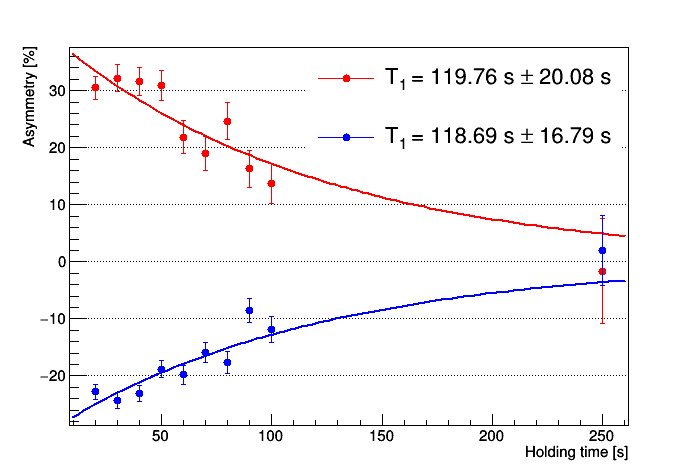
\includegraphics[width=\textwidth]{figures/ramsey2017_t1.png}
  \vspace{8pt}
  \caption{}\label{subfig:ramsey2017_t1_asymmetry}
\end{subfigure}%DO NOT REMOVE THIS '%'
\begin{subfigure}{.5\textwidth}
  \centering
  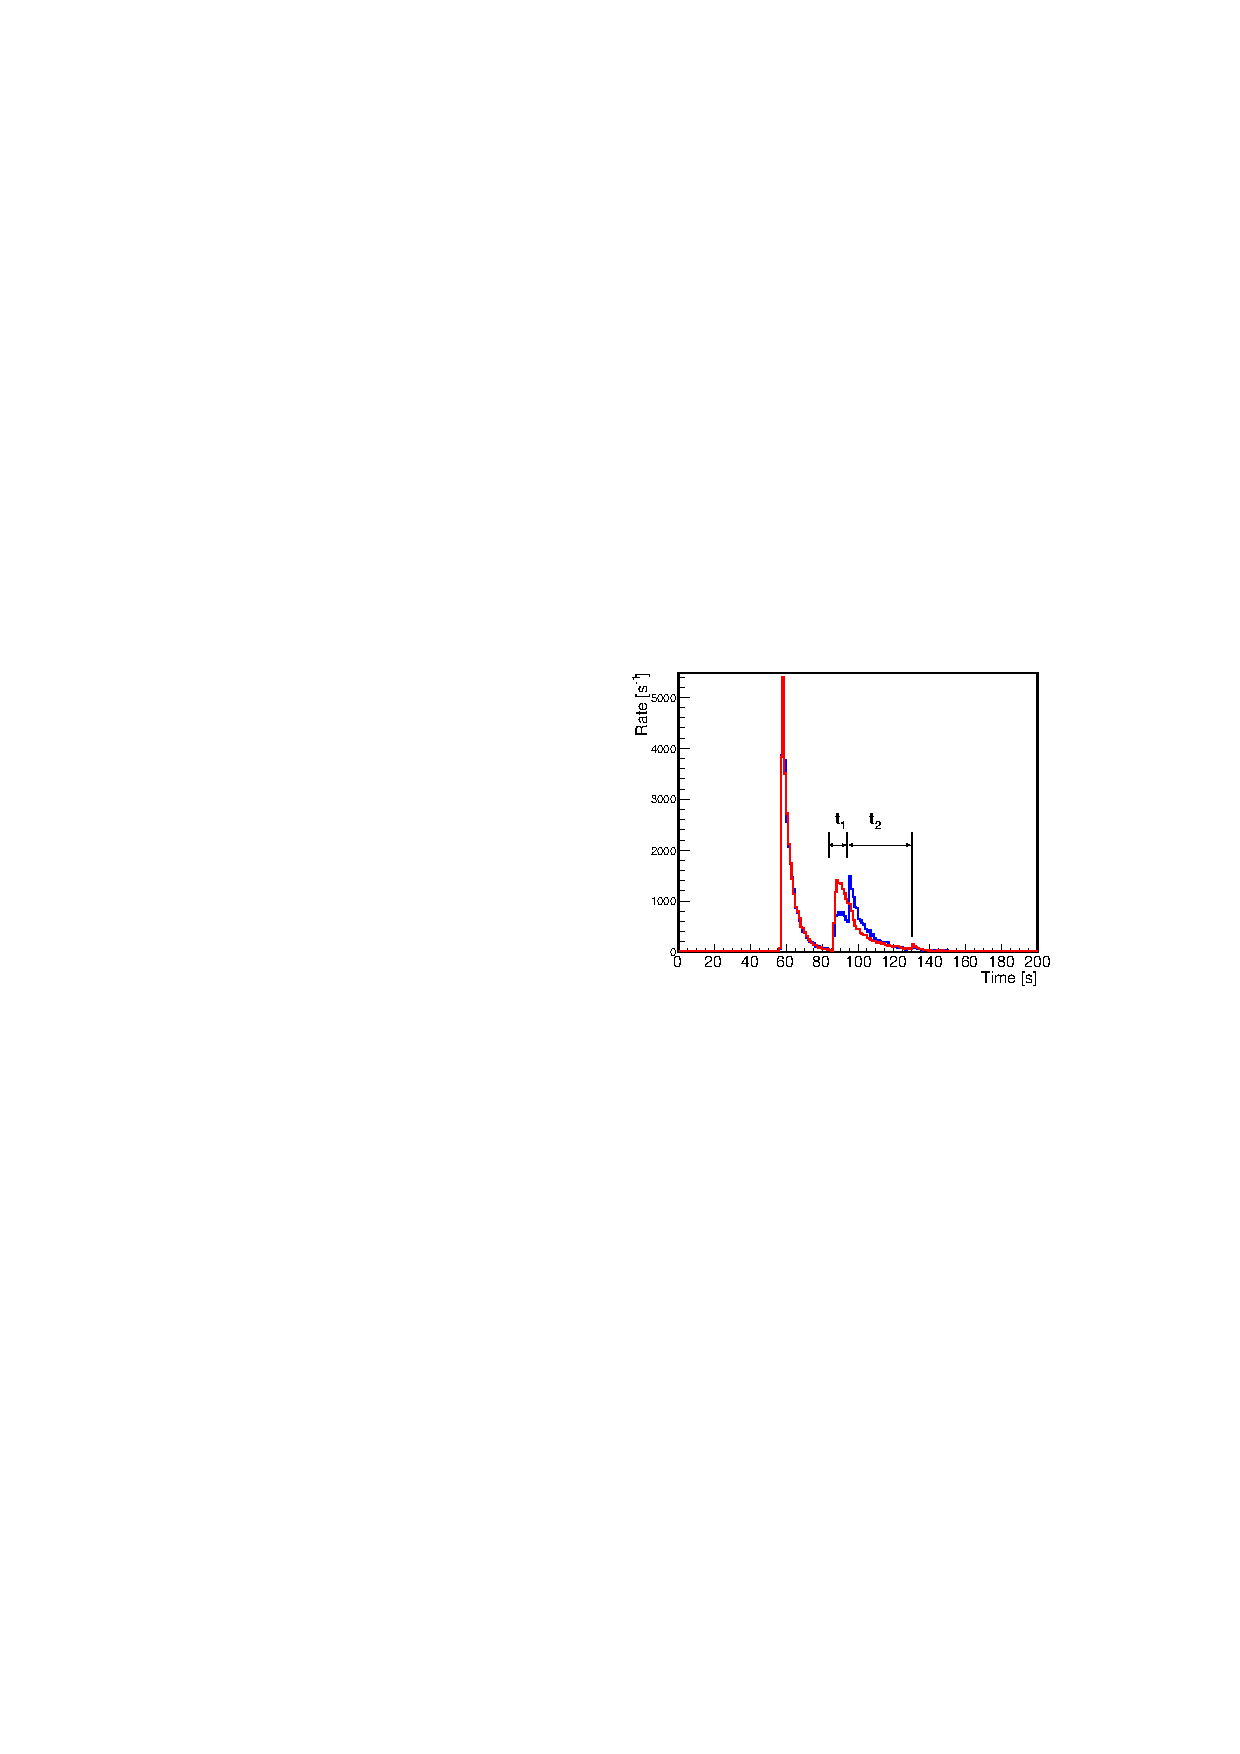
\includegraphics[width=\textwidth]{figures/ramsey_2017_t1_measurement_pair.pdf}
  \caption{}\label{subfig:ramsey2017_t1_doublet}
\end{subfigure}
\caption
    [Spin asymmetry as a function of holding time in the prototype apparatus.]
    {\textbf{(\subref{subfig:ramsey2017_t1_asymmetry})} Spin asymmetry as a function of holding time in the prototype apparatus. The red line refers to asymmetry during counting period $t_1$, and the blue line refers to asymmetry measured during counting period $t_2$. A fit of the measurements with a decaying exponential gives longitudinal spin relaxation time $T_1$. \textbf{(\subref{subfig:ramsey2017_t1_doublet})} Neutron count rate from a fill-and-dump run doublet. The red line refers to the sequence with the spin flipper toggling off-on-off during the cell dump, and blue refers to a on-off-on sequence. Figures by Robert Pattie Jr.}
\label{fig:ramsey_2017_t1}
\end{figure}

A measurement of longitudinal relaxation time $T_1$ (Sec.~\ref{sec:spin_relaxation}) was taken using the fill-and-dump sequence from Sec.~\ref{subsec:holdingTimeMeasurement} (Fig.~\ref{fig:timeSpectrum}). The preload period was \qty{45}{\second}, and the filling period was \qty{5}{\second}. Filling time was kept short to limit depolarization opportunity for \ucn in the guide system.

Storage times were varied from \qty{30}{\second} to \qty{250}{\second}. For each storage time parameter, two fill-and-dump runs (a ``run doublet'') with different counting sequences were performed. During the \qty{65}{\second} counting period, the spin flipper was off (on) for $t_1=\qty{10}{s}$, on (off) for $t_2=\qty{35}{s}$, and off (on) for \qty{20}{\second}. Figure~\ref{subfig:ramsey2017_t1_doublet} shows neutron count rate from a fill-and-dump run doublet with the labeled integration periods $t_1$ and $t_2$.

For an integration period $t_i$, the asymmetry $A_i$ is given by
%
\begin{gather}
    A_i=\frac{\Gamma_{\text{on, }i}-\Gamma_{\text{off, }i}}{\Gamma_{\text{on, }i}+\Gamma_{\text{off, }i}}
    \label{eq:spin_asymmetry} 
\end{gather}
%
where $\Gamma_i$ is the normalized number of UCN counted in the corresponding integration period, and the on/off subscript refers to the spin flipper state during $t_1$. Detector counts were normalized using the preload count rate on the West beamline monitor as per the procedure in Sec.~\ref{subsec:dataProcessing}. No cell valve leak was observed in the data from the 2017 measurement cycle. For holding times $<\qty{40}{s}$, the guide dump (Sec.~\ref{subsec:dataProcessing}) did not complete before the start of the counting period. In these cases, the guide dump was fit with a decaying exponential. The fit was then integrated over the counting period and was subtracted.

Assymetry (for both $t_1$ and $t_2$) as a function of storage time is shown in Fig.~\ref{subfig:ramsey2017_t1_asymmetry}. A fit of the measurements with a decaying exponential $A(t)=A_0\exp(-t/T_1)$ gives longitudinal spin relaxation time $T_1$. Fitting both curves Fig.~\ref{subfig:ramsey2017_t1_asymmetry} and calculating the average gave $\langle T_1 \rangle=\qty{199(13)}{s}$. 

In the limit $t=0$ (effectively 0 storage time), we have $A(0)\approx 0.3$. By comparison, a direct flow through mode measurement from the \ucn source to the drop detector (Fig.~\ref{fig:spin_flipper_efficiency}) gives $A(0)\approx 0.8$. In addition, changing the cell wall from dPS cell wall to NiP did not significantly change $T_1$, suggesting that the spin relaxation time was mostly the result of magnetic field gradients.

The gradient $\partial B_0 / \partial z$ in a precession cell can be estimated from $T_1$ using Eq.~(\ref{eq:T1_dBdZ_mcgregor}) (assuming no contribution to depolarization from wall bounces). We take the mean wall collision time $\tau_\text{c}=4V/(\bar{v}A)=\qty{36.7}{ms}$ (Appx.~\ref{appx:ucn_effusion}). This gives $\partial B_0/\partial z\approx \qty{12}{\micro G\per cm}$. At the time no in situ measurement method was available to confirm field gradient. It is likely that a stainless steel bellows in the prototype apparatus responsible for cell valve actuation was the source of the gradient. The bellows was replaced with a nonmagnetic version immediately after the 2017 measurement cycle.

%%%%%%%%%%%%%%%%%%%%%%%%%%%%%%%%%%%%%%%%%%%%%%

\section{Rabi measurement}\label{sec:2017_rabi_measurement}

%%%%%%%%%%%%%%%%%%%%%%%%%%%%%%%%%%%%%%%%%%%%%%

\begin{figure}
    \centering
    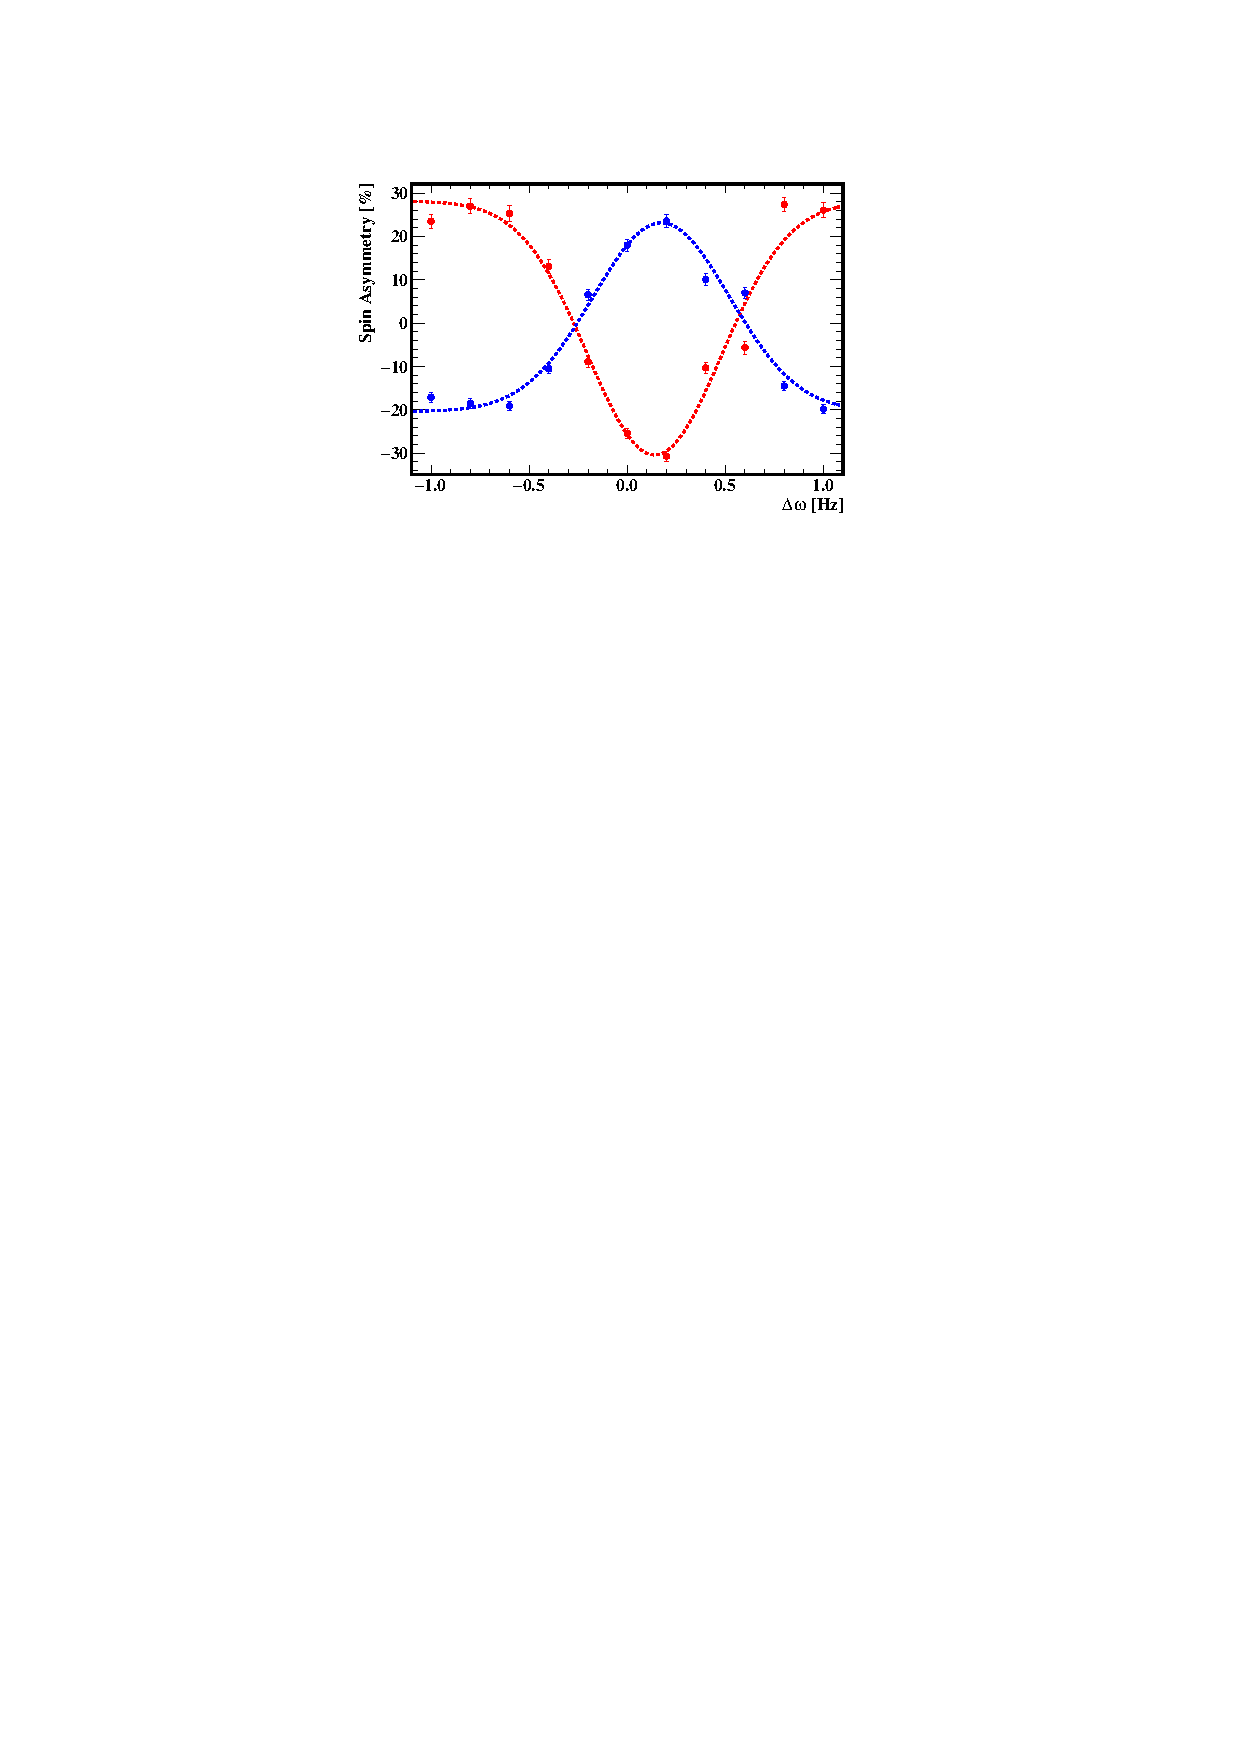
\includegraphics[width=0.55\textwidth]{figures/2017_rabi_fringe.pdf}
    \caption
    [Rabi fringe measured in the prototype apparatus.]
    {Rabi fringe measured in the prototype apparatus. A plot of spin asymmetry (\ref{eq:spin_asymmetry}) as a function of $\pi$ pulse frequency. Figure by Robert Pattie Jr.}
    \label{fig:rabi_fringe_2017}
\end{figure}

A Rabi fringe (Fig.~\ref{fig:rabi_fringe_2017}) was produced using the same run sequence as the $T_1$ measurements, with a \qty{30}{\second} storage time. \qty{5}{\second} after the start of the storage period, a \qty{1}{\second}-long $\pi$ pulse was applied. The frequency range of the Rabi fringe was $\qty{64.5}{Hz} \pm \qty{1}{Hz}$ with step size \qty{0.2}{Hz}. The spin asymmetry at each frequency step was calculated using Eq.~(\ref{eq:spin_asymmetry}). The fit of the Rabi fringe gave a resonant frequency of \qty{0.17(1)}{Hz}, with a full width half maximum of \qty{0.8(1)}{Hz}.

%%%%%%%%%%%%%%%%%%%%%%%%%%%%%%%%%%%%%%%%%%%%%%

\section{Ramsey measurement}\label{sec:2017_ramsey_measurement}

%%%%%%%%%%%%%%%%%%%%%%%%%%%%%%%%%%%%%%%%%%%%%%

Ramsey fringes (Fig.~\ref{fig:ramsey_fringes_2017}a--\ref{fig:ramsey_fringes_2017}c) were created with the same run parameters as the Rabi sequence, with two $\pi/2$ pulses each with duration \qty{0.5}{s} each. Three different precession times were used ($\gls*{T_fp}=\qty{1}{s},\,\qty{10}{s},\,\qty{20}{s}$). The total storage time was held constant at \qty{30}{\second}.

Spin asymmetry was calculated with the same procedure as Sec.~\ref{sec:2017_rabi_measurement}, and the maximal spin asymmetry for each Ramsey fringe was determined by fitting the fringe (see Eqs.~(\ref{eq:neutrons_in_ramsey_seq}) and (\ref{eq:four_point_ramsey_fringe_fit})). A plot of max asymmetry as a function of free precession period is shown in Fig.~\ref{fig:ramsey_fringes_2017}d. We see that as \gls*{T_fp} has increased max asymmetry has decreased, which means that as \ucn are allowed to precess for longer periods of time the transverse spin gets increasingly relaxed. Therefore fitting a decaying exponential to the data in Fig.~\ref{fig:ramsey_fringes_2017}d is a measure of transverse relaxation time. This was found to be $T_2=\qty{19.5(2.7)}{s}$.

From Eq.~(\ref{eq:T2_mcgregor}) (again assuming negligible depolarization from wall bounces) we estimated the transverse gradient in the cell. We let diffusion constant $D_\text{ucn}\approx \qty{2.2}{m^2 \per s}$~\cite{golubUCN} from Eq.~(\ref{eq:ucn_diffusion_constant}), using the assumption that the chance of a diffuse reflection in the cell is of order $\sim 10\%$. Therefore, assuming transverse gradients along $x$ and $y$ are of roughly equally magnitude, we find $\partial B_z/\partial r \approx \qty{18}{\micro G \per cm}$. This is consistent with the estimate obtained in Sec.~\ref{sec:2017_t1_measurement}.

%%%%%%%%%%%%%%%%%%%%%%%%%%%%%%%%%%%%%%%%%%%%%%

\section{Pulse sequence instrumentation}

%%%%%%%%%%%%%%%%%%%%%%%%%%%%%%%%%%%%%%%%%%%%%%

The $\pi$ and $\pi/2$ pulses in Secs.~\ref{sec:2017_rabi_measurement}--\ref{sec:2017_ramsey_measurement} used a SRS DS345 with its amplitude modulated by a DG535 pulse generator. The precision of these devices in the context of the LANL nEDM experiment is discussed in Sec.~\ref{sec:pulse_gen_freq_std}. Appendix~\ref{appx:gpib_usb_pulse_sequence} provides the code used to set the pulse sequencing for the Rabi and Ramsey fringe measurements in this chapter.

\vspace{\baselineskip}

\begin{figure}[hbp]
    \centering
    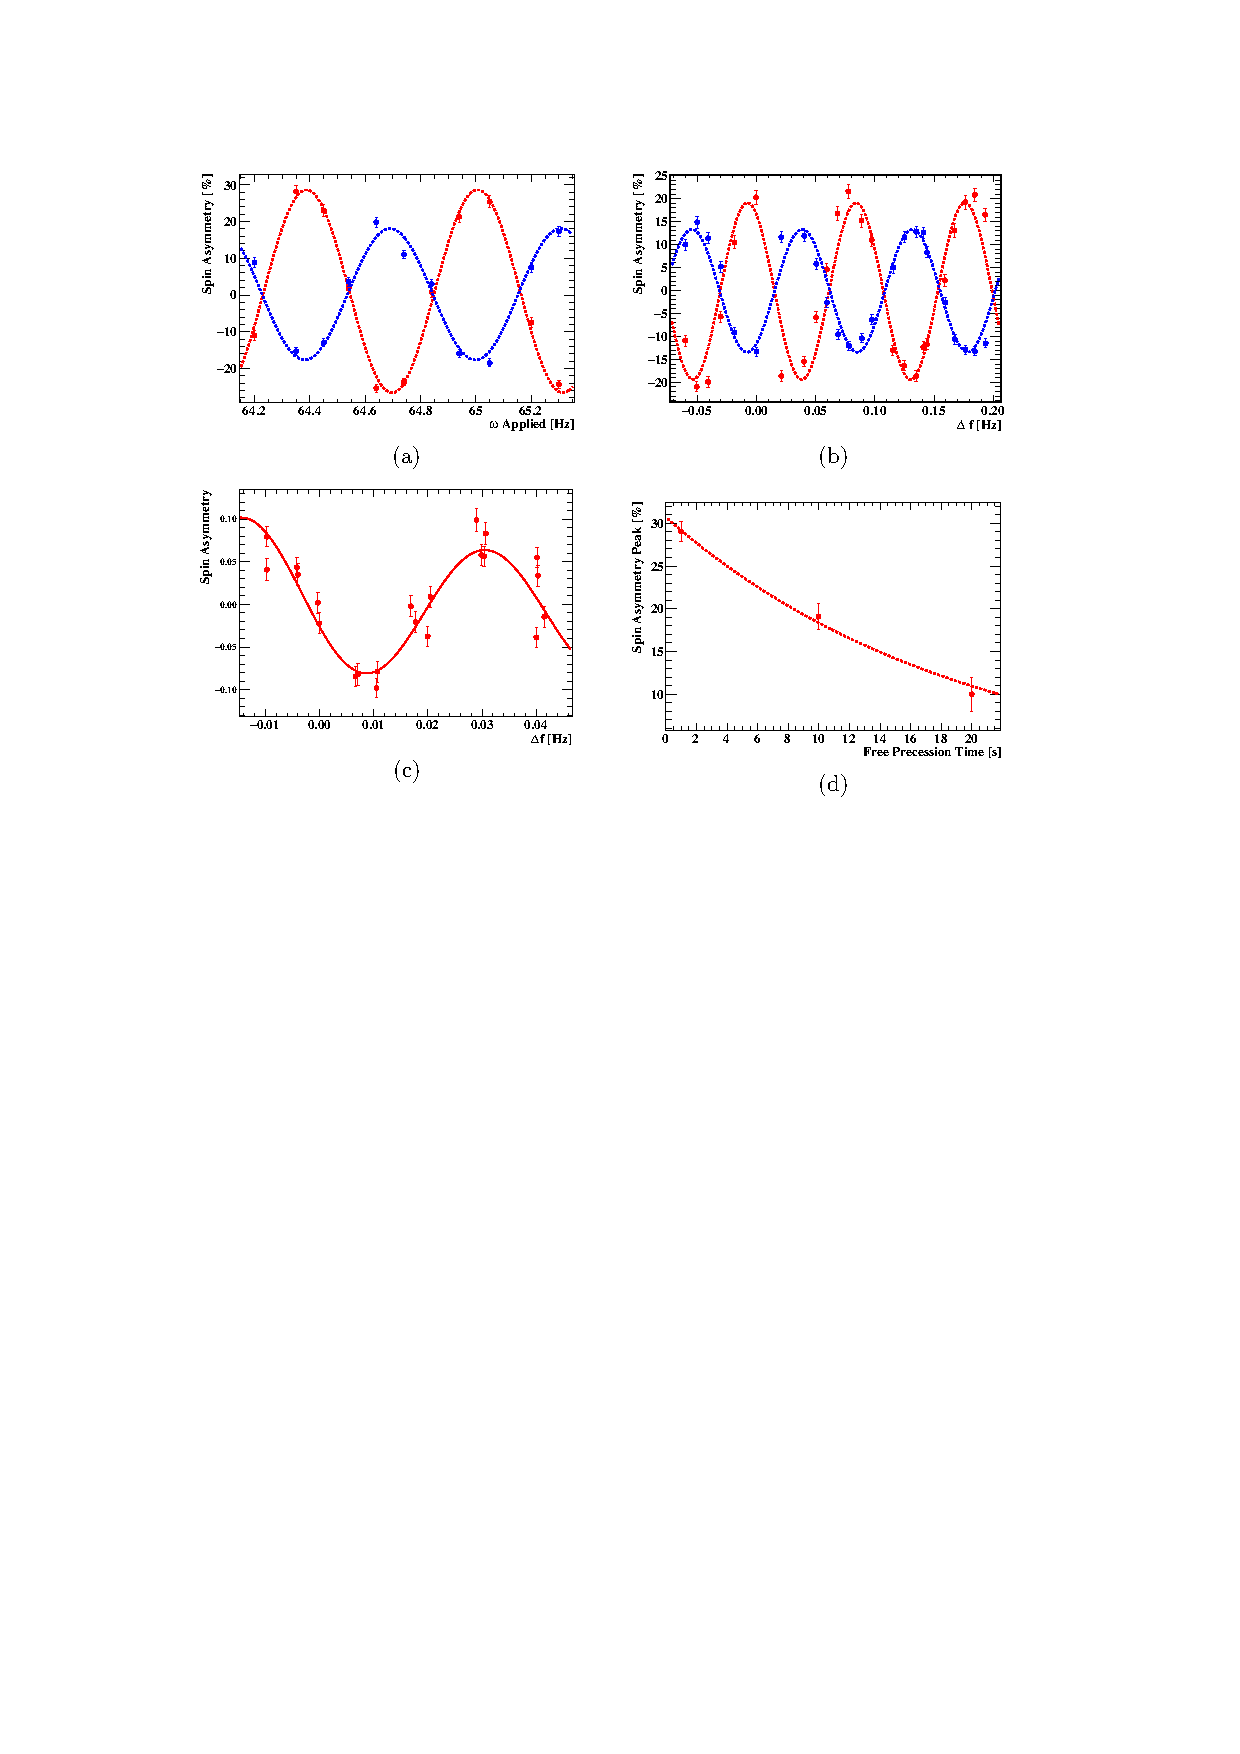
\includegraphics[width=\textwidth]{figures/2017_ramsey_fringes.pdf}
    \caption
    [Ramsey fringes measured in the prototype apparatus.]
    {Ramsey fringes measured in the prototype apparatus. Free precession period $\gls*{T_fp}=\text{\textbf{(a)} }\qty{1}{s}$, \text{\textbf{ (b)} }$\qty{10}{s}$, \text{\textbf{ (c)} }$\qty{20}{s}$. Panel \textbf{(d)} shows a fit to the maximal spin asymmetry of each fringe (\ref{eq:spin_asymmetry}) as a function of \gls*{T_fp}. A fit of \textbf{(d)} with a decaying exponential gives $T_2=\qty{19.5(2.7)}{s}$. Figures provided by Robert Pattie Jr. and Takeyasu Ito.}
    \label{fig:ramsey_fringes_2017}
\end{figure}